\documentclass{article}
\usepackage[affil-it]{authblk}
\usepackage{listings}
% Language setting
% Replace `english' with e.g. `spanish' to change the document language
\usepackage[english]{babel}
\usepackage{enumitem}

% Set page size and margins
% Replace `letterpaper' with`a4paper' for UK/EU standard size
%\usepackage[letterpaper,top=2cm,bottom=2cm,left=3cm,right=3cm,marginparwidth=1.75cm]{geometry}
\usepackage[a4paper,top=2cm,bottom=2cm,left=3cm,right=3cm,marginparwidth=1.75cm]{geometry}

% Useful packages
\usepackage{amsmath}
\usepackage{graphicx}
\usepackage{caption}
\usepackage{subcaption}
\usepackage[colorlinks=true, allcolors=blue]{hyperref}

%\title{\includegraphics[width=0.3\textwidth]{rino2.jpg}  \hspace*{2cm} \Huge{RINO User Manual}  }
\title{\includegraphics[scale=0.4]{rino2.jpg} \\  \Huge{RINO User Manual}  }
\author{Eric Goubault and Sylvie Putot}
\affil{LIX, Ecole Polytechnique, CNRS and Institut Polytechnique de Paris,  \\91128
Palaiseau, France \\ name.surname@polytechnique.edu}


\begin{document}



\maketitle



\begin{abstract}
We present the C++ RINO library, available on \url{https://github.com/cosynus-lix/RINO/},  for the computation of inner and outer approximations of reachable sets for uncertain discrete-time or continous-time dynamical systems, with (possibly time-varying) disturbances and control inputs, where some of the control inputs can be specified as outputs of a neural network.

For continuous-time systems, it relies on Taylor expansions in time and affine arithmetic (i.e. zonotopes) in space based reachability analysis to compute outer envelopes of all possible trajectories of an uncertain system. Additionally, it uses a generalized mean-value theorem to deduce inner tubes, that contain only states guaranteed to be reached. It also studies robust versions of these tubes, when there can be control inputs and perturbations to the system. Finally, the control can be specified as the output of a neural network which inputs are the system state.
\end{abstract}

%%%%%%%%%%%%%%%%%%%%%%%%%%%%%%%%%%%%%%%%%

\section{Introduction and references}
 RINO implements the following:
\begin{itemize}[noitemsep]
\item Forward inner and outer-approximated reachability of non-linear differential systems~\cite{hscc2017}.  The reachability algorithm relies on Taylor expansions in time and affine arithmetic (i.e. zonotopes) in space for computing over or outer-approximating tubes.  Under or inner-approximating tubes are deduced by application of a generalized mean-value theorem to the flow of the system.  This supposes to compute an over-approximation of the solution flow and its Jacobian with respect to uncertain inputs and initial conditions.
\item Forward inner and outer-approximated reachability of non-linear delay differential systems with constant delay~\cite{cav18}.  Using the classical method of steps,  the problem is reduced to the reachability analysis of a sequence of non-linear differential systems. 
\item Robust inner and outer approximations of differential systems with possibly time-varying disturbances~\cite{hscc19}: the above reachability analysis is extended to the case with both disturbances and control inputs.
\item In \cite{hscc2017,cav18,hscc19},  inner-approximations are computed for one-dimensional projections.  RINO also implements vector-valued inner-approximations~\cite{lcss2020}. (in practice, 2 and 3-dimensional projections).
\item In \cite{hscc2017,cav18,hscc19,lcss2020}, the under-approximation relies on a mean-value theorem, which may be imprecise in some cases.  In~\cite{adhs21}, higher-order inner-approximations are proposed.  They are implemented in RINO in the case of discrete-time dynamical systems.   
\item In \cite{hscc2017,cav18,hscc19,lcss2020,adhs21}, the control inputs are specified either in a range (for constant or piecewise constant inputs) or as solution of a differential system (for differentiable time-varying inputs).  Some of the control inputs can also be specified as the output of a neural network taking as input the system state~\cite{cav22}. This constitutes neural network controlled systems.  In RINO, the underlying dynamical system can be either discrete-time or continuous time.  For the time being, the activation functions have to be differentiable functions (typically sigmoid and hyperbolic tangent). 



\end{itemize}
%%%%%%%%%%%%%%%%%%%%%%%%%%%%%%%%%%%%%%%%%
\section{Installation}

\subsection{Using docker}

Get the RINO directory and run 
\begin{verbatim}
$ docker build .
\end{verbatim}
An image \texttt{shaxyz...}  is built which you can run by 
\begin{verbatim}
$ docker run -it --name rino shaxyz.... 
\end{verbatim}
You can then execute RINO from directory /home/RINO as described in Section \ref{running}.

\subsection{Building from sources}

%\setlist{nolistsep}

\begin{itemize}[noitemsep]

\item You need g++, LAPACK and BLAS installed. Python visualization was tested with Python 3.8.8. 

\item Install the FILIB++ Interval Library, available from \url{http://www2.math.uni-wuppertal.de/wrswt/software/filib.html} (we used Version 3.0.2), and set variable \$FILIBHOME

\item Get and unzip the FADBAD++ automatic diffentiation package, available from \url{http://www.fadbad.com/fadbad.html} (we used FADBAD++ 2.1), and set variable \$FADBADHOME.
Copy files fadbad.h and fadiff.h from RINO/FADBAD\_Modified/ into your FADBAD++ distribution (we modified these files to add differentiation of activation functions).

\item A slightly modified of the third party package for Affine Arithmetic aaflib-0.1 (\url{http://aaflib.sourceforge.net}) has been included in the current directory. 
Future plans include separating more cleanly the initial version and our modifications...
Go to directory aaflib-0.1 within the current package and compile by "make static". 

\item Returning to the main (RINO) directory, you can now compile by "make" and obtain the "main" executable. 
\end{itemize}
The installation has been mostly tested on MacOS, but should also work on Ubuntu. 

%%%%%%%%%%%%%%%%%%%%%%%%%%%%%%%%%%%%%%%%%

\section{Running the reachability analysis \label{running}}

For now, the dynamics of systems on which to perform reachability analysis are defined as C++ code and given a fixed id used to run their analysis:
\begin{itemize}[noitemsep]
\item  for ODEs and DDEs in ```ode\_def.h``` (system and constant parameters) and ```ode\_def.cpp``` (parameters, initial conditions and input ranges)
\item for discrete-time systems in ```discrete\_system.h``` and ```discrete\_system.cpp``` 
  \end{itemize}
Running an example is then performed at command line, in directory /home/RINO, by 
\begin{verbatim}
$ ./rino [-systype system_type -syschoice system_id] [-nnfile-sfx nnfile.sfx] 
[-configfile cfgfile.txt]
\end{verbatim}
where 
\begin{itemize}[noitemsep]
\item \texttt{system\_type} is either \texttt{ode} (for a system of Ordinary Differential Equations) or \texttt{dde} (for a system of Delay Differential Equations) or \texttt{discrete} (for a discrete-time dynamical system)
\item \texttt{system\_id} is an integer specifying the predefined system identifier (matching variable syschoice in file ode\_def.h for ODEs and DDEs and  discrete\_system.h for discrete-time systems )
\item \texttt{nnfile.sfx}  contains a neural network in the Sherlock \texttt{sfx} format (\url{https://github.com/souradeep-111/sherlock/blob/master/sherlock-network-format.pdf}) 
\item \texttt{cfgfile.txt} specifies analysis parameters,  inputs,  initial conditions of the system.  
\end{itemize}

Note that default values for parameters, inputs and initial conditions of the system are set in the code.  If a configuration file is used,  the configuration file values override those present in the code. 

At command line,  either the system type and choice should be specified, or a configuration file containing this information should be provided.  If both are provided,  the configuration file information overrides command-line options.  Finally,  the  name of file containing the neural network, when relevant,  can be provided either at command-line or in the configuration file. 

The parameters which can be set in the configuration file are described in Section \ref{params}.  The commands for running the different examples presented in our work are given in Section \ref{existing}.

%The examples of neural network files are in directory ```Examples/Networks```.

\subsection{Running existing systems \label{existing}}

\subsubsection{Continuous-time differential systems (ODEs)}

\begin{itemize}[noitemsep]
\item The Brusselator example~\cite{hscc2017} (the system is an ODE and is given syschoice identifiant equal to 2) is run by:
\begin{verbatim}
$./rino -systype ode -syschoice 2
\end{verbatim}
or if you want to use a configuration file to modify the parameter and initial conditions, by:
  \begin{verbatim}
$./rino -configfile Examples/ConfigFiles/cfg_ode_2.txt
\end{verbatim}
In what follows,  we will use the following aggregate notation to indicate these two alternatives:
  \begin{verbatim}
$./rino -systype ode -syschoice 2 [-configfile Examples/ConfigFiles/cfg_ode_2.txt]
\end{verbatim}
\item The self-driving car example \cite{hscc19}  is run by 
 \begin{verbatim}
$./rino -systype ode -syschoice 6 [-configfile Examples/ConfigFiles/cfg_ode_6.txt]
\end{verbatim}
% or  \begin{verbatim}
%$ ./rino -configfile Examples/ConfigFiles/cfg_ode_6.txt
% \end{verbatim}
% \item the crazyflie model of Reference [HSCC 2019]  is run by "./rino -systype ode -syschoice 18 [Examples/ConfigFiles/cfg_ode_18.txt]" )
  \end{itemize}
  
\subsubsection{Continuous-time delay differential systems with constant delays (DDEs)}
\begin{itemize}[noitemsep]
\item  The running example of \cite{cav18} is run  by 
\begin{verbatim}
$./rino -systype dde -syschoice 1 [-configfile Examples/ConfigFiles/cfg_dde_1.txt]
\end{verbatim}
\item  Example 10 of \cite{cav18} is run  by 
\begin{verbatim}
$./rino -systype dde -syschoice 3 [-configfile Examples/ConfigFiles/cfg_dde_3.txt]
\end{verbatim}
\item  Example 9 (self-driving car with uncertain PID coefficients) of \cite{cav18} is run  by 
\begin{verbatim}
$./rino -systype dde -syschoice 8 [-configfile Examples/ConfigFiles/cfg_dde_8.txt]
\end{verbatim}
\item  The platoon examples of \cite{cav18} are run, for 5 vehicles by 
\begin{verbatim}
$./rino -systype dde -syschoice 10 [-configfile Examples/ConfigFiles/cfg_dde_10.txt]
\end{verbatim}
or for 10 vehicles by: 
\begin{verbatim}
$./rino -systype dde -syschoice 11 [-configfile Examples/ConfigFiles/cfg_dde_11.txt]
\end{verbatim}
 \end{itemize}

\subsubsection{Discrete-time dynamical systems}
\begin{itemize}[noitemsep]
\item the test model of \cite{adhs21} with Algorithm 1 is run by 
\begin{verbatim}
$./rino -systype discrete -syschoice 15 -nbsteps 25 [-iter_method 1] 
[-AEextension_order 1] [-skew 1]
\end{verbatim} 
or equivalently
\begin{verbatim}
$./rino -configfile Examples/ConfigFiles/cfg_discrete_15.txt
\end{verbatim}
\item the SIR epidemic model of \cite{adhs21} with Algorithm 1 (Fig. 3) is run by 
\begin{verbatim}
$./rino -configfile Examples/ConfigFiles/cfg_discrete_16_1.txt
\end{verbatim} 
and the same model with different initial conditions and Algorithm 2 (Fig. 4) is run by  
\begin{verbatim}
$./rino -configfile Examples/ConfigFiles/cfg_discrete_16_2.txt
\end{verbatim}
\item the Honeybees Site Choice Model \cite{adhs21} with Algorithm 2 is run by 
\begin{verbatim}
$./rino -configfile Examples/ConfigFiles/cfg_discrete_17.txt
\end{verbatim}
 \end{itemize}
 
\subsubsection{Neural network controlled dynamical systems (continuous or discrete time) \label{nnex}}
The  examples of ~\cite{cav22} can be run by
\begin{itemize}[noitemsep]
\item TORA:
\begin{verbatim}
$./rino -configfile Examples/ConfigFiles/cfg_tora_tanh.txt
$./rino -configfile Examples/ConfigFiles/cfg_tora_sigmoid.txt
\end{verbatim}
\item B1:
\begin{verbatim}
$./rino -configfile Examples/ConfigFiles/cfg_B1_tanh.txt
$./rino -configfile Examples/ConfigFiles/cfg_B1_sigmoid.txt
\end{verbatim}
\item B2
\begin{verbatim}
$./rino -configfile Examples/ConfigFiles/cfg_B2_sigmoid.txt
\end{verbatim}
\item B3
\begin{verbatim}
$./rino -configfile Examples/ConfigFiles/cfg_B3_tanh.txt
$./rino -configfile Examples/ConfigFiles/cfg_B3_sigmoid.txt
\end{verbatim}
\item B4:
\begin{verbatim}
$./rino -configfile Examples/ConfigFiles/cfg_B4_tanh.txt
$./rino -configfile Examples/ConfigFiles/cfg_B4_sigmoid.txt
\end{verbatim}
\item B5:
\begin{verbatim}
$./rino -configfile Examples/ConfigFiles/cfg_B5_tanh.txt
$./rino -configfile Examples/ConfigFiles/cfg_B5_sigmoid.txt
\end{verbatim}
\item ACC:
\begin{verbatim}
$./rino -configfile Examples/ConfigFiles/cfg_acc_tanh.txt
\end{verbatim}
\item Continuous-time Mountain Car
\begin{verbatim}
$./rino -configfile Examples/ConfigFiles/cfg_MC_sigmoid.txt
\end{verbatim}
\item Discrete-time Mountain Car
\begin{verbatim}
$./rino -configfile Examples/ConfigFiles/cfg_discrete_mc.txt
\end{verbatim}
\end{itemize}
\subsection{Adding one's own example}
In short (to be completed, but a lot of additional information can already be found in Section~\ref{params} and \ref{examples}):
\begin{itemize}[noitemsep]
\item For ODEs,  the dynamical system should be given an (unused) syschoice ID and the dynamics defined in file \texttt{ode\_def.h}, in class OdeFunc,  by the vector yp  of time derivatives as function of state vector y and possibly parameters.  

The dimension of the state vector (sysdim) needs to be set in file \texttt{ode\_def.cpp} in function define\_system\_dim(). The parameters and initial values (if not given at command line in a configuration file) need to be set in function init\_system() in the same file. 

\item For discrete-time systems, the process is very similar but in a different location. Give the system  an (unused) syschoice ID and define the dynamics in file \texttt{discrete\_system.h}, in class DiscreteFunc, by the vector z of next discrete state as a function of the current state x and possibly parameters. 
The dimension of the state vector (sysdim) and the initial conditions need to be set in file \texttt{discrete\_system.h}  in function init\_discrete\_system().  
\end{itemize}
Both continuous-time and discrete-time systems can take (see also Sections \ref{params} and \ref{examples})
\begin{itemize}[noitemsep]
\item constant but possibly uncertain parameters (vector variable \texttt{params} in the C++ code),
\item constant or piecewise constant control inputs or disturbances (vector variable \texttt{param\_inputs} in the C++ code),
\item control inputs defined as the output of a neural network which input is the system state  (vector variable \texttt{control\_inputs} in the C++ code).
\end{itemize}
%%%%%%%%%%%%%%%%%%%%%%%%%%%%%%%%%%%%%%%%%


\section{Parameters of analysis and Configuration File \label{params}}
We list in this section the parameters and inputs of the system that can be set in the configuration file.  All of these parameters have default values in the program, so that they may be ommitted in the configuration file. 
For examples of use, we refer the reader to:
\begin{itemize}[noitemsep]
\item Section~\ref{existing} for sample files (in directory Examples/ConfigFiles) for existing examples,
\item Section~\ref{examples} for fully detailed results on chosen examples.
\end{itemize}
\subsection{Parameters of the analysis common to all system types \label{common}}

\paragraph{System definition}
\begin{itemize}
\item Keyword \texttt{systype}: class of dynamical system, can be equal to \texttt{ode, dde, discrete}.  For example:
\begin{verbatim}
systype = ode
\end{verbatim}

\item Keyword \texttt{syschoice}: identifier for dynamical system,  should be equal to an integer, and matched by a system definition in RINO.
\begin{itemize}
\item if systype is \texttt{ode}, the dynamics of the system should be defined in   \texttt{ode\_def.h}, in class OdeFunc,  by the vector yp  of time derivatives as function of state vector y and possibly system parameters, 
\item if systype is \texttt{dde}, the dynamics of the system should be defined in   \texttt{ode\_def.h}, in class DdeFunc,  by the vector yp  of time derivatives as function of state vector y and delayed state vector y\_prev,  and possibly parameters,
\item if systype is \texttt{discrete},  the dynamics should be defined in \texttt{discrete\_system.h}, in class DiscreteFunc, by the vector z of next discrete state as a function of the current state x and possibly system parameters. 
\end{itemize}
Note that the same syschoice identifier can be used (with different system definition) for different values of systype.  
For example:
\begin{verbatim}
syschoice = 2
\end{verbatim}
\end{itemize}

\paragraph{Uncertain inputs and initial conditions}
\begin{itemize}
\item Keyword \texttt{initial-values}: should be equal to a sequence of intervals separated by a white space, which length is the dimension of the system (equal to global variable \texttt{sysdim} in the code).  The cartesian product of these intervals defines the set of initial values of the dynamical system, whatever its type. 
For example:
\begin{verbatim}
initial-values = [-0.1,0.1] [0,0.1] [1.9,2.1] [2.9,3.1]
\end{verbatim}
In cases when the accuracy of analysis is not considered sufficient, it can be refined by partitioning one component of the initial domain (for the time being, only one component at at time can be partitioned).  
You can specify the component you want to subdivide and the number of partitions. For example,  for 2 subdivisions for the last component: 
\begin{verbatim}
initial-values = [-0.1,0.1] [0,0.1] [1.9,2.1] ([2.9,3.1],2) 
\end{verbatim}
[***Warning***: the partitioning functionality is implemented only for systype ode and dde and has not been tested recently] 

\item Keyword \texttt{inputs}: for constant but uncertain inputs,  should be equal to a sequence of  intervals separated by a white space,  which length is the dimension of the input vector (equal to global variable \texttt{inputsdim} in the code). In class OdeFunc, the variable name for these inputs is \texttt{param\_inputs}.
For example:
\begin{verbatim}
inputs = [-0.1,0.1] [-0.1,0.1]
\end{verbatim}
For piecewise constant inputs,  one can specify the number of pieces for the piecewise constant function over the time horizon.  A constant input period is supposed.
For example, for an input which first component is constant and second component is piecewise constant with 10 pieces:
\begin{verbatim}
inputs = ([-0.1,0.1],1) ([-0.1,0.1],10) # same as inputs = [-0.1,0.1] ([-0.1,0.1],10)
\end{verbatim}

\item Keyword \texttt{uncontrolled}: should be equal to a sequence of integers which length is smaller or equal to the dimension of the input vector. It defines which dimensions of the inputs (numbered starting from 1) are disturbances, the remaining dimensions being considered as control inputs.
For example,  if the first 2 dimensions of the input vectors are disturbances:
\begin{verbatim}
uncontrolled = 1 2
\end{verbatim}


\item Keyword \texttt{params}: should be equal to  a sequence of  intervals separated by a white space,  which length is the dimension of the vector of uncertain but constant parameters (equal to global variable  \texttt{paramsdim} in the code).  In class OdeFunc, the variable name for these parameters is \texttt{params}.
For example:
\begin{verbatim}
params = [2,2] [3,4]
\end{verbatim}
Parameters are handled differently from inputs in the definition of the robust reachable sets~\cite{hscc19}.  In particular,  they don't add dimensions to the Jacobian matrix of the trajectories, used to compute the robust under and over-appproximations. 
\end{itemize}

\paragraph{Analysis}
\begin{itemize}
\item Keyword \texttt{refined-mean-value}: should be 0 or 1,  depending whether a coarse mean-value theorem is implemented for under-approximation, using the Jacobian evaluation for all input intervals (refined-mean-value=0), or a refined version (see e.g. Theorem 1 in \cite{lcss2020}).
\begin{verbatim}
refined-mean-value = 1
\end{verbatim}
The improvement due to this refined formula have been disappointing compared to the complexity of implementation, so that this option will probably be deprecated in further versions. 
\end{itemize}

\paragraph{Output results and visualization}
\begin{itemize}
\item Keyword \texttt{samples-per-dim}: should be an integer defining the number of samples in each input dimension used  for reachable set estimation by trajectory samples.  The samples are used  to compute estimated ranges for each state variable and to print sample points at different integration time steps of the analysis.
For example:
\begin{verbatim}
samples-per-dim = 20
\end{verbatim}

\item Keyword \texttt{create-png}: should be 0 or 1. If 0, the visualization script is not called by the analysis (in which case only the data file are produced,  the visualization script can be run a posteriori, see Section \ref{visu}).
For example, for not calling the visualization script:
\begin{verbatim}
create-png = 0
\end{verbatim}

\item Keyword \texttt{interactive-visualization}: should be 0 or 1.  If 0,  the figures are only saved in the output directory (provided create-png is 1), otherwise they are also plotted on screen. 
For example:
\begin{verbatim}
interactive-visualization = 1
\end{verbatim}

\item Keyword \texttt{points-per-graph}: should be an integer specifying the number of time points saved in the output files and printed on graphs. This is disconnected from the analysis time steps, and only means that the state may not be saved for all time steps, for better lisibility. 
For example:
\begin{verbatim}
points-per-graph = 50
\end{verbatim}

\item Keyword \texttt{variables-to-display}: should be a sequence of integer greater or equal to 1 indicating the dimensions we wish to visualize graphically (the data output files will still be produced for all dimensions). This is useful for examples of large dimensions when all dimensions may not be meaningful. 
For example:
\begin{verbatim}
variables-to-display = 1 2
\end{verbatim}
If we want to display figures for all dimensions (which is the default when the option is not set in the config file):
\begin{verbatim}
variables-to-display = all
\end{verbatim}
\end{itemize}

\subsection{Parameters common to ODEs and DDEs (systype is ode or dde) \label{odedde}}


Additionally to the parameters of Section~\ref{common},  for both ODEs and DDEs, the following parameters can be tuned:
\begin{itemize}
\item Keyword \texttt{time-horizon}: a real number  defining the time horizon of the reachability analysis (note that for DDEs the starting time can be tuned, while for ODEs it is equal to 0).
For example:
\begin{verbatim}
time-horizon = 5.
\end{verbatim}
\item Keyword \texttt{order}: an integer specifying the order for Taylor expansions in time on each time step. 
For example:
\begin{verbatim}
order = 3
\end{verbatim}

\end{itemize}

\subsection{Parameters specific to ODEs (systype is ode)}

Additionally to the parameters of Sections~\ref{common} and \ref{odedde}, in the case of ODEs the following parameter can be tuned:
\begin{itemize}
\item Keyword \texttt{integration-step}: a real number defining the time step of Taylor models in the reachability analysis (no variable time steps for the time being)
\begin{verbatim}
integration-step = 0.02
\end{verbatim}
\end{itemize}
\subsection{Parameters specific to DDEs (systype is dde)}

Additionally to the parameters of Sections~\ref{common} and \ref{odedde}, in the case of DDEs the following parameters can be tuned:
\begin{itemize}
\item Keyword \texttt{starting-time}: a real number specifying the initial time of definition of the initial conditions (for ODEs, the initial conditions are given at time 0).  Often in the examples, this initial time is the opposite of the delay value,  with initial conditions defined between the starting time and 0, and integration starting at time 0. 
For example:
\begin{verbatim}
starting-time = -0.3
\end{verbatim}
\item Keyword \texttt{delay}: the constant delay in the DDE. 
For example:
\begin{verbatim}
delay = 0.3 
\end{verbatim}
\item Keyword \texttt{nb-time-subdivisions}: an integer which defines the integration time step by the delay divided by nb-time-subdivisions. (this replaces the definition of integration-step of ODEs).
For example:
\begin{verbatim}
nb-time-subdivisions = 3
\end{verbatim}
\end{itemize}

\subsection{Parameters specific to discrete-time systems (systype is discrete)}
Additionally to the parameters of Section~\ref{common}, in the case of discrete-time systems, the following parameters can be tuned:
\begin{itemize}
\item Keyword \texttt{nbsteps}: an integer specifying the number of discrete time steps.
For example:
\begin{verbatim}
nbsteps = 25
\end{verbatim}
\item Keyword \texttt{iter-method}: should be either 1 or 2,  specifying whether Algorithm 1 or 2 in \cite{adhs21} is used for iterated discrete-time reachability.  
For example:
\begin{verbatim}
iter-method = 1
\end{verbatim}
\item Keyword \texttt{skew}: should be either 0 or 1, specifying whether boxes or skewed boxes (linear transform of a box) should be used for the approximation of vector valued functions: this choice influences the precision in Algorithm 1 (this vector-valued approximation is used as initial condition of the next discrete time step) while it is only used for visualization in Algorithm 2.
In the general case,  a value of 1 (skewed box) is recommended. Only in a very few  cases, the preconditioning linear transform may possibly degrade the approximation. 
For example:
\begin{verbatim}
skew = 1
\end{verbatim}
\item Keyword \texttt{AEextension-order}: should be either 1 or 2,  respectively specifying that a first-order (mean-value) or a 2nd order~\cite{adhs21} (Taylor model) approximation will be used for under and robust approximations. 
For example:
\begin{verbatim}
AEextension-order = 1
\end{verbatim}
\end{itemize}

\subsection{Parameters specific to neural network controlled dynamical systems (systype can be either ode or discrete)}

Both ODEs and discrete-time systems can have control components defined as the output of a neural network (it should work for DDEs as well but has not been tested).  In this case, additionally to the parameters of ODEs or discrete-time systems,  the user can specify the following:
\begin{itemize}
\item Keyword \texttt{nnfile-sfx}: specifies the file containing the neural network.  It is given for now in the Sherlock sfx format (\url{https://github.com/souradeep-111/sherlock/blob/master/sherlock-network-format.pdf}). 
For example:
\begin{verbatim}
nnfile-sfx = Examples/Networks/tora_tanh.sfx
\end{verbatim}
Note that we are currently working on onnx format integration, we hope to make the possibility available soon.
\item Keywords \texttt{nn-offset} and \texttt{nn-scaling}: in some cases in the related work,  the output \texttt{control\_inputs} of the network is transformed to give the control as follows:
\begin{verbatim}
 nn_scaling_factor*(control_inputs[0]-nn_offset)
\end{verbatim}
These  final offset and scaling of the network output can be specified in the configuration file.
For example:
\begin{verbatim}
nn-offset = 0. # also read at the end of sfx file if present (erasing this one)
nn-scaling = 11.  # also read at the end of sfx file  if present (erasing this one)
\end{verbatim}
\item Keyword \texttt{control-step}: a real nuber specifying the period at which the neural network is evaluated on the current step to give a new control value,  which then remains constant on the whole control step. 
For example:
\begin{verbatim}
control-step = 0.1
\end{verbatim}
\end{itemize}
%%%%%%%%%%%%%%%%%%%%%%%%%%%%%%%%%%%%%%%%%


\section{Visualizing results \label{visu}}

\paragraph{Analysis output files}
After running an example, all results are in the subdirectory ‘output’. They are provided in the following files : 
\begin{itemize}[noitemsep]
\item \texttt{sumup.txt}: summary of configuration, running time and ranges at the final state of the analysis (part of this information can also be found with more significant digits in \texttt{sumup.yaml})
\item \texttt{samplesreachset.yaml}: sampled trajectories (used to assess accuracy of reachability results)
\item \texttt{approxreachset.yaml}: over and under-approximated reachset (projected, robust, joint ranges) and accuracy measures (eta, gamma) at each time step 
\end{itemize}

\paragraph{Running the visualization script}
A python visualization file \texttt{Visu\_output.py} is available in the GUI directory. It can be run from the analyzer (if variable create-png is set to 1 in the configuration file) but you can also run it separately,  provided the above data files are present in RINO/output.  It may even be required if you are running the docker version (see below the pararaph docker specifics).

For example, for an interactive analysis (prints the figures on screen, otherwise the files are simply saved in the output directory) and to produce figures only for variables x[1] and x[2]),  it is run by:
\begin{verbatim}
$cd GUI; python3 Visu_output.py --interactive=1 --printvar=-1-2; cd ..
\end{verbatim}
When the script is run by analyzer, the options set above in command line can be set in the configuration file by: 
\begin{verbatim}
interactive-visualization = 1
variables-to-display = 1 2
\end{verbatim}
\paragraph{One-dimensional projections}
%The files produced may slightly vary depending on the system type. (ode, dde, discrete-time).
For k ranging from 1 to system dimension, the following results files display the projected ranges on dimension k as function of time:
\begin{itemize}[noitemsep]
\item \texttt{xk\_max.png}  (e.g.  \texttt{x1\_max.png})  and \texttt{xk\_max\_sample.png}: the maximal inner and outer-approximations, with and without sampled trajectories
\item \texttt{xk.png},  \texttt{xk\_sample.png}: additionally to the maximal inner and outer-approximations, the robust approximations when relevant, with and without sampled trajectories
\end{itemize}
Global views are provided: \texttt{xi\_max.png} and \texttt{xi\_subplots\_min\_max.png} display the one-dimensional projected reachable sets for all variables on one graph. 

\paragraph{Two and three-dimensional projections}
For any couple (k,l) we also display 2-dimensional projections:
\begin{itemize}[noitemsep]
\item \texttt{xkxl.png}:  maximal (and when relevant robust~\cite{hscc19}) inner and outer-approximations of the joint or vector-valued range (xk,xl) as skewed boxes. (see e.g. ~\cite{lcss2020})
\item \texttt{xkxl\_sample.png}: sampled trajectories for (xk,xl) 
\item \texttt{xkxl\_approx\_sample.png}: on the same graph the inner and outer-approximations of the joint range (xk,xl) as skewed boxes and sampled trajectories
\item \texttt{xkxl\_box\_sample.png}: same as above but the approximations are printed as boxes (useful in a few cases where the skewed boxes have a bad behavior)
\item \texttt{xkxl\_finalstate.png}: box and skewed box inner and outer-approximations, robust when relevant, and sampled points at the final state of the analysis
\end{itemize}
Three-dimensional projections when relevant are also printed, only the corners of boxes are printed for more lisibility.

\paragraph{Error measures}
We display the following error measures (the closer to 1 the better) as functions of time (or iterations for discrete-time systems) in files \texttt{eta.png},  \texttt{gamma.png}: for the projection on each state variable, we define $\eta_o$ = (width of sampled set)/(width of outer-approx) ; $\eta_i$ = (width of inner-approx)/(width of sampled set);
$\gamma$ = (width of inner-approx)/(width of outer-approx).

\paragraph{Docker specifics}

It is rather difficult under docker to ensure that the visualization on the host
machine will go correctly without further machine-dependant local installations.
We can then turn off the automatic visualization in the configuration files 
and rely on a local execution of a python script file on the
host machine for generating the figures, as having a python installation working
on the host machine is much easier to ensure than the link between docker and
a X11 interface.

First, you have to make sure that you have an \texttt{output} directory under the \texttt{\$HOME/RINO} directory on the host machine (not under the docker container): 
\begin{verbatim}
> mkdir output
\end{verbatim}

Then for instance for retrieving on the host machine the elements after analysis needed for visualization on the host machine, you will need to type in a console on the host machine:

\begin{verbatim}
> cd $HOME/RINO/output
> docker cp rino:/home/RINO/output/approxreachset.yaml . 
> docker cp rino:/home/RINO/output/samplesreachset.yaml .
> docker cp rino:/home/RINO/output/sumup.txt .
> docker cp rino:/home/RINO/output/sumup.yaml .
\end{verbatim}


Then for visualization (make sure \texttt{python3} is installed on your host machine - the scripts have been run successfully with python 3.6 to 3.8), you can e.g. write: 
\begin{verbatim}
> cd ../GUI ; python3 Visu_output.py --interactive=0 --printvar=-1-2 ; cd ../output ; ls
eta.png
gamma.png
x1.png
x1_max.png
x1_max_sample.png
x1_sample.png
xi_max.png
xi_subplots_max.png
(...)
\end{verbatim}

%%%%%%%%%%%%%%%%%%%%%%%%%%%%%%%%%%%%%%%%%
\section{Examples \label{examples}}

To be completed. 

\subsection{Neural network controlled ODE (example B1)}

We describe here the example named B1 in Section~\ref{nnex} of a neural network controlled continuous-time dynamical system,  called for instance with a neural network with sigmoid activation functions.  
It is called by
\begin{verbatim}
$./rino -configfile Examples/ConfigFiles/cfg_B1_sigmoid.txt
\end{verbatim}

\subsubsection{Configuration file and system definition and initialization}
The contents of the configuration file \texttt{cfg\_B1\_sigmoid.txt} are as follows:
\begin{verbatim}
# B1 sigmoid (sys 471)
systype = ode
syschoice = 471
nnfile-sfx = Examples/Networks/B1_sigmoid.sfx
nn-offset = 0.5. # also read from nn file (erasing this one)
nn-scaling = 8.  # also read from nn file (erasing this one)
time-horizon = 7.
control-step = 0.2
integration-step = 0.05
order = 3
initial-values = [0.8,0.9] [0.5,0.6]
create-png = 0
\end{verbatim}
First note that not all possible parameters are set  in this configuration file,  default values are taken for the others. 
\paragraph{System definition}
The system is a continuous-time dynamical system (\texttt{systype=ode}),  the system ID is 471 (\texttt{syschoice = 471}). 
The definition of this system can be found in file \texttt{ode\_def.h} in class \texttt{OdeFunc} by looking for ID 471:
\small
\lstset {language=C++}
\begin{lstlisting}
class OdeFunc {
  template <class C> void operator()(vector<C> &yp, vector<C> params, 
  vector<C> param_inputs, vector<C> control_inputs, vector<C> y) { 
   [...]      
    else if (syschoice == 471) {
      yp[0] = y[1];
      yp[1] = (nn_scaling_factor*(control_inputs[0]-nn_offset))*(y[1]*y[1])-y[0];
    }
   [...]
\end{lstlisting}
\normalsize
This function defines the dynamic of the system by its time derivative.  In the present case,  it defines:
 \[ 
 \begin{array}{l} \dot x_1  = x_2 \\
              \dot x_2 = u x_2^2 - x_1 \end{array} 
\]
In this example, there are no constant parameters (params) and no uncertain inputs or disturbances (param\_inputs).  There is however a control given as an affine transform of the output \texttt{control\_inputs[0]} of a neural network controller:
\[ u := \mbox{ nn\_scaling\_factor*(control\_inputs[0]-nn\_offset) }\]
The neural network controller in sfx file is described in file \texttt{Examples/Networks/B1\_sigmoid.sfx} as described by the \texttt{nnfile-sfx} line in the configuration file. The offset and scaling factors are also read from the configuration file (\texttt{nn-offset = 0.5} and \texttt{nn-scaling = 8}).

Note that this definition of the system complemented in the C++ file \texttt{ode\_def.cpp} by the specification of the systems dimension in function void \texttt{define\_system\_dim():}
\small
\lstset {language=C++}
\begin{lstlisting}
void define_system_dim() {
[...]
 else if (syschoice == 471) {  
    sysdim = 2;
    inputsdim = 0;
    nncontroldim = 1;
 }
[...]
\end{lstlisting}
\normalsize
The system dimension is 2 ($x_1$ and $x_2$), the inputs dimension is 0 (no uncertain inputs or disturbances), and there is one control defined as the output of a neural network controller.

\paragraph{System initialization and analysis parameters}
The initial values for $x_1$ and $x_2$ at time 0 are given in box $[0.8,0.9] \times [0.5,0.6]$, as specified by the line starting with \texttt{initial-values} in the configuration file.  
The time step is 0.05, the control period is 0.2, and the time horizon is 7.  The analysis will be performed with Taylor models of order 3 in time on each time step. 
These settings, as specified by the configuration file,  override the (same here) values that may have been set in \texttt{ode\_def.cpp}, in function 

\small
\lstset {language=C++}
\begin{lstlisting}
void init_system()
[...]
  else if (syschoice == 471) {  
      tau = 0.05; 
      t_end = 7.;  
      Taylor_order = 3;
      initial_values[0] = interval(0.8,0.9);
      initial_values[1] = interval(0.5,0.6);
      control_period = 0.2;
  }
  [...]
\end{lstlisting}
\normalsize     

\subsubsection{Results and visualization}
\paragraph{Running the analysis}
When running the example by 
\begin{verbatim}
>./rino -configfile Examples/ConfigFiles/cfg_B1_sigmoid.txt
\end{verbatim}
the analysis should output something like:
\small
 \begin{verbatim}
 ****** Reading system choice from file Examples/ConfigFiles/cfg_B1_sigmoid.txt ******
nn_scaling_factor =8reading network fromExamples/Networks/B1_sigmoid.sfx
nn_offset=0.5
nn_scaling_factor=8
nb_inputs layer 0 = 2 nb_outputs = 20 activation function = 1
nb_inputs layer 1 = 20 nb_outputs = 20 activation function = 1
nb_inputs layer 2 = 20 nb_outputs = 1 activation function = 1
inputsdim=0sysdim=2
****** Reading system parameter from file Examples/ConfigFiles/cfg_B1_sigmoid.txt ******
initial_value=[0.8, 0.9]
initial_value=[0.5, 0.6]
****** End parameter reading ******

fullinputsdim=0
mv: rename output to output_sauv/output: Directory not empty
Estimate reachset:
Estimated reachable set at tn = 0.05 is: z[0]=[0.824021, 0.928744]  z[1]=[0.456494, 0.553304]  
Estimated reachable set at tn = 0.1 is: z[0]=[0.846037, 0.954955]  z[1]=[0.411477, 0.506155]  
Estimated reachable set at tn = 0.15 is: z[0]=[0.865984, 0.978606]  z[1]=[0.365086, 0.458601]  
Estimated reachable set at tn = 0.2 is: z[0]=[0.883804, 0.99967]  z[1]=[0.317469, 0.410684]  
Estimated reachable set at tn = 0.25 is: z[0]=[0.89955, 1.01831]  z[1]=[0.272649, 0.369659]  
Estimated reachable set at tn = 0.3 is: z[0]=[0.913247, 1.03463]  z[1]=[0.225815, 0.32679]  
Estimated reachable set at tn = 0.35 is: z[0]=[0.924809, 1.04854]  z[1]=[0.177268, 0.282256]  
Estimated reachable set at tn = 0.4 is: z[0]=[0.934162, 1.05994]  z[1]=[0.127347, 0.236258]  
Estimated reachable set at tn = 0.45 is: z[0]=[0.941242, 1.06877]  z[1]=[0.0764235, 0.189017]  
Estimated reachable set at tn = 0.5 is: z[0]=[0.946015, 1.075]  z[1]=[0.0250271, 0.142152]  

[...]
[...]
[...]

Estimated reachable set at tn = 7 is: z[0]=[0.108126, 0.14668]  z[1]=[0.175081, 0.195133]  
At t=0 :
x[0]=[0.8, 0.9]	x[1]=[0.5, 0.6]	

nncontrol[i]=[0.452, 0.526]
setting new bf at time 0
without quadrature: Xouter=z[0]=[0.824, 0.929] z[1]=[0.451, 0.56] 
Xinner=z[0]=[0.824, 0.929] z[1]=[0.463, 0.549] 
with intersection with direct solution: t=0.05
Xouter_maximal[0]=[0.824002, 0.928773] 	Xinner_maximal[0]=[0.824095, 0.928696] Sampled estim.[0]=[0.824021, 0.928744] 	 eta_o[0]=0.999548	 eta_i[0]=0.998832	 gamma[0]=0.99838
Xouter_maximal[1]=[0.45599, 0.554644] 	Xinner_maximal[1]=[0.462626, 0.548631] Sampled estim.[1]=[0.456494, 0.553304] 	 eta_o[1]=0.981313	 eta_i[1]=0.888394	 gamma[1]=0.871792

[...]
[...]
[...]

without quadrature: Xouter=z[0]=[0.0962, 0.159] z[1]=[0.164, 0.209] 
Xinner=z[0]=[0.121, 0.134] z[1]=[ EMPTY ] 
with intersection with direct solution: t=7
Xouter_maximal[0]=[0.101547, 0.153317] 	Xinner_maximal[0]=[0.120924, 0.133972] Sampled estim.[0]=[0.108126, 0.14668] 	 eta_o[0]=0.744716	 eta_i[0]=0.338445	 gamma[0]=0.252046
Xouter_maximal[1]=[0.171882, 0.20041] 	Xinner_maximal[1]=[nan, nan] 	Sampled estim.[1]=[0.175081, 0.195133] 	 eta_o[1]=0.702897	 eta_i[1]=nan	 gamma[1]=nan

elapsed time (sec) =0.589801
......
Result files are in the output directory
Visualize them with by : cd GUI; python3 Visu_output.py --interactive=0 --printvar=all; cd ..
The python script will save files as png files (in same directory output)
 \end{verbatim}
 \normalsize
This output corresponds to the following steps:
\begin{itemize}[noitemsep]
\item it starts by reading the configuration file and the neural network,
\item it  computes some sample trajectories to estimate the reachable set width at each time step, with same time step as for reachability analysis (the individual points of trajectories are output in the \texttt{samplesreachset.yaml} output file),
\item it performs the reachability and outputs at each time step projections of under and over-approximations and error measures (eta and gamma); these results are also saved in the \texttt{approxreachset.yaml} output file,
\item the final results at the end of the time horizon (here t=7) are printed in the \texttt{sumup.txt} output file.
\end{itemize}
All files can be found in the \texttt{output} directory.  For example, here, opening  \texttt{output/sumup.txt}:
\small
\begin{verbatim}
-----------------------------------------------------------------------------------------------
                           Summary   
                      Command-line   ./rino -configfile Examples/ConfigFiles/cfg_B1_sigmoid.txt 
----------------------------------------------------------------------------------------------- 
                           Systype | ode
                          Dynamics | 471
                Initial conditions | [0.8, 0.9] [0.5, 0.6] 

                            Inputs | 
                     Time interval | [0,7]
                      Control step  | 0.2
                         Time step | 0.05
                  System dimension  |  2
               Taylor Models order |  3
               Neural network file  |  Examples/Networks/B1_sigmoid.sfx
----------------------------------------------------------------------------------------------
Sampled estimate of final reachset |  [0.108, 0.147] [0.175, 0.195] 
                Over-approximation  | [0.102, 0.153] [0.172, 0.2] 
               Under-approximation |  [0.121, 0.134] [ EMPTY ] 
----------------------------------------------------------------------------------------------
       Elapsed analysis time (sec)  |  0.589801
       Elapsed sampling time (sec) | 2.02754
\end{verbatim}
\normalsize
%\section{Authors and References}

%%%%%%%%%%%%%%%%%%%%%%%%%%%%%%%%%%%%%%%%%

\paragraph{Visualization}
You can visualize the  reachability results by running the following  from the RINO directory, provided the results files are in RINO/output (see Section \ref{visu} and in particular paragraph Docker specifics if running under docker):
\begin{verbatim}
>cd GUI; python3 Visu_output.py --interactive=0 --printvar=all; cd ..
\end{verbatim}
Listing files in the output directory produces:
\small
\begin{verbatim}
approxreachset.yaml    x1.png                 x1x2_box_sample.png    x2_sample.png
eta.png                x1_max.png             x1x2_finalstate.png    xi_max.png
gamma.png              x1_max_sample.png      x1x2_sample.png        xi_subplots_max.png
samplesreachset.yaml   x1_sample.png          x2.png
sumup.txt              x1x2.png               x2_max.png
sumup.yaml             x1x2_approx_sample.png x2_max_sample.png

\end{verbatim}
\normalsize
The dimension of this system being equal to 2,  projections are computed for x1 and x2, and joint approximations for x1 and x2. 
In this example,   there are no inputs which can be seen as disturbances or controls,  thus the robust and maximal reachable sets are identical, and pictures x1.png  and x1\_max.png are identical, and so are x1\_sample.png  and x1\_max\_sample.png (similarly for x2).  Figure~\ref{fig:Proj_B1} shows the projected reachable sets on each component x1 and x2: the filled blue region is the under-approximation of the reachable set, while the plain black lines give the outside bounds of the over-approximation. 
\begin{figure}[htbp]
\centering
\begin{subfigure}{.5\textwidth}
  \centering
  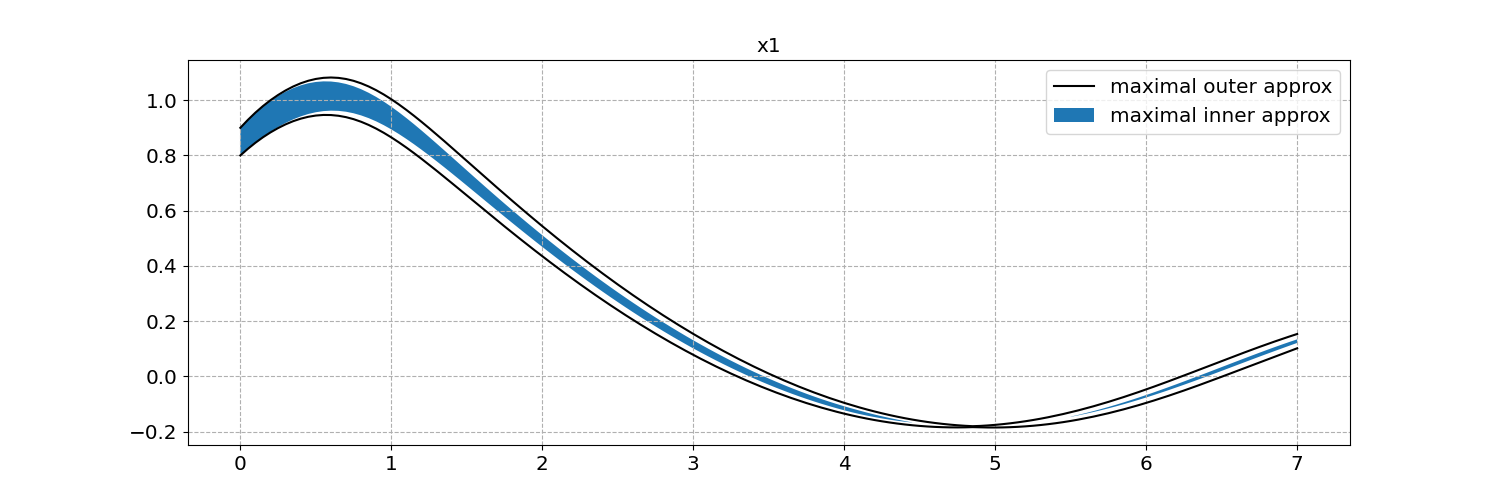
\includegraphics[width=.99\linewidth]{x1_B1sig.png}
  \caption{x1.png}
  \label{fig:sub1}
\end{subfigure}%
\begin{subfigure}{.5\textwidth}
  \centering
  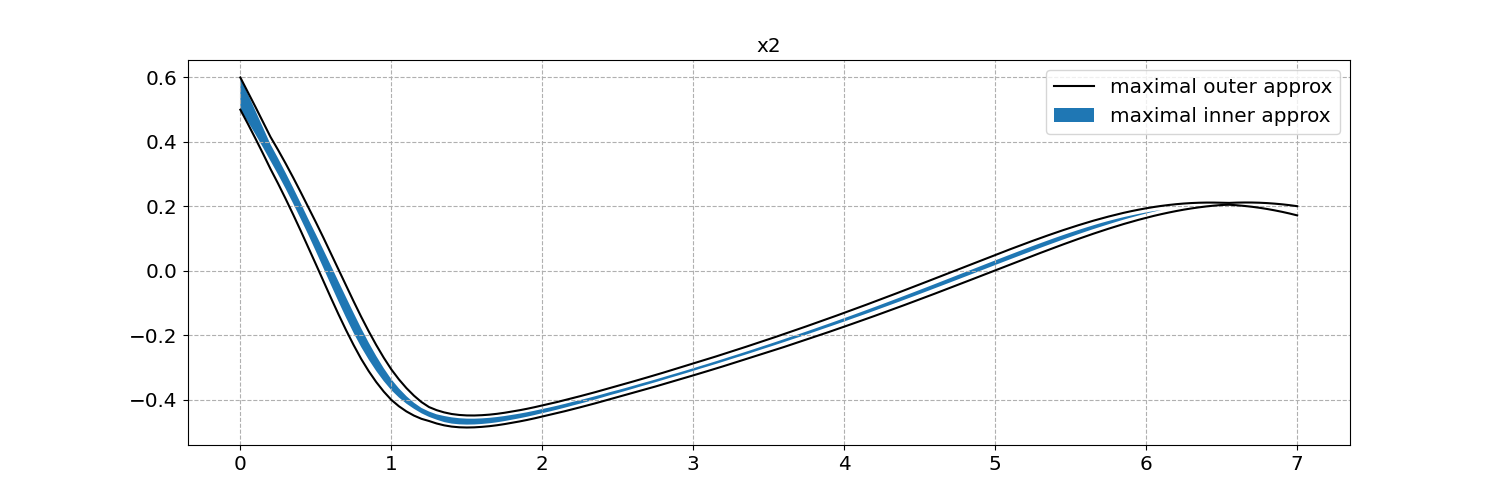
\includegraphics[width=.99\linewidth]{x2_B1sig.png}
  \caption{x2.png}
  \label{fig:sub2}
\end{subfigure}
\caption{Projected under and over-approximations for the B1 example with sigmoid network (cfg\_B1\_sigmoid.txt)}
\label{fig:Proj_B1}
\end{figure}
In Figure~\ref{fig:Proj_sample_B1}, the  approximations of the reachable set for x1 is printed together with (in purple dots) points of sampled trajectories.  The number of sample trajectories can be parameterized in the configuration file.  
\begin{figure}[htbp]
\centering
  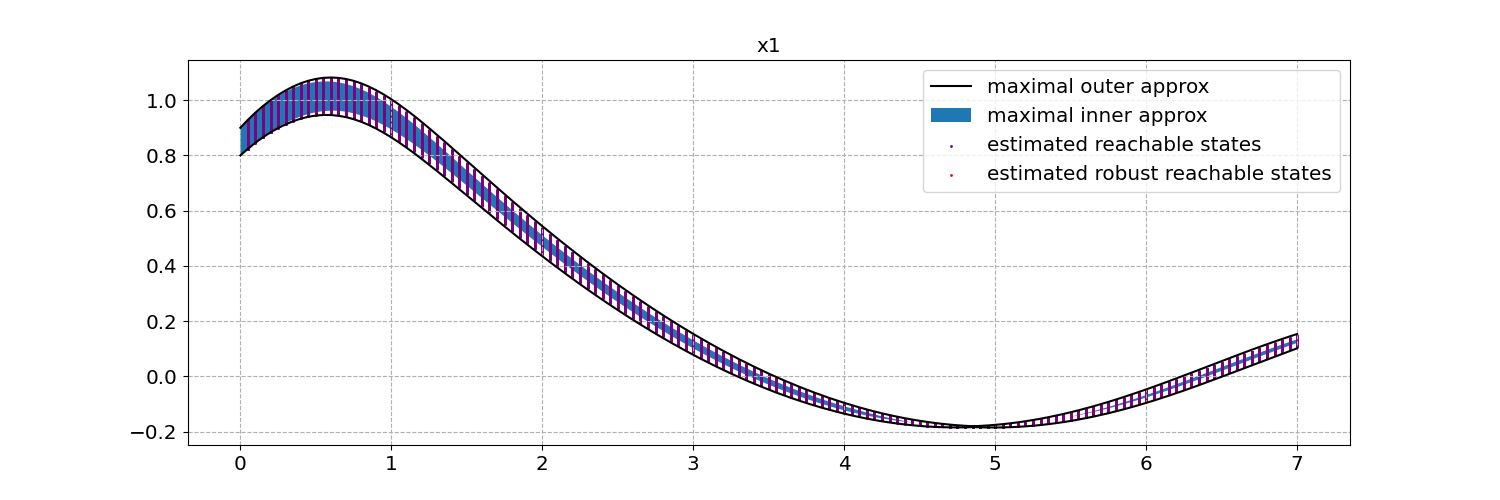
\includegraphics[width=.99\linewidth]{x1_sample_B1sig.png}
\caption{ x1\_sample.png for the B1 example}
\label{fig:Proj_sample_B1}
\end{figure}
The 2-dimensional under (in orange) and over-approximations (in green) together with sample points (in purple) are printed at each time step in Figure~\ref{fig:Proj_sample_B1}. The initial state is the yellow square in the upper right quarter. First note that for the over-approximation, we don't represent exactly the zonotope  computed at each time step, by evaluation of the Taylor model with zonotopic coefficients, but a skewed box over-approximation of this zonotope.  Note also that the cartesian product of the projected under-approximation on each component is not an under-approximation of the (2-dimensional) vector-valued function, but we have an algorithm to compute box or skewed box under-approximations as well, see e.g. ~\cite{lcss2020,adhs21}. Finally, at some point in the iterations, the precodnitioning which gives the directions of the skewed boxes can be no longer meaningful, after which we print boxes instead, as the result of a heuristics.  This is what happens here in the last part of the trajectories when green boxes are printed, which appear much less accurate than the skewed boxes printed at previous iterates (the heuristics probably still needs some calibration...). However remember that this loss of precision is only for printing, what is propagated is the underlying zonotopes which we approximate by these skewed boxes.  
\begin{figure}[htbp]
\centering
  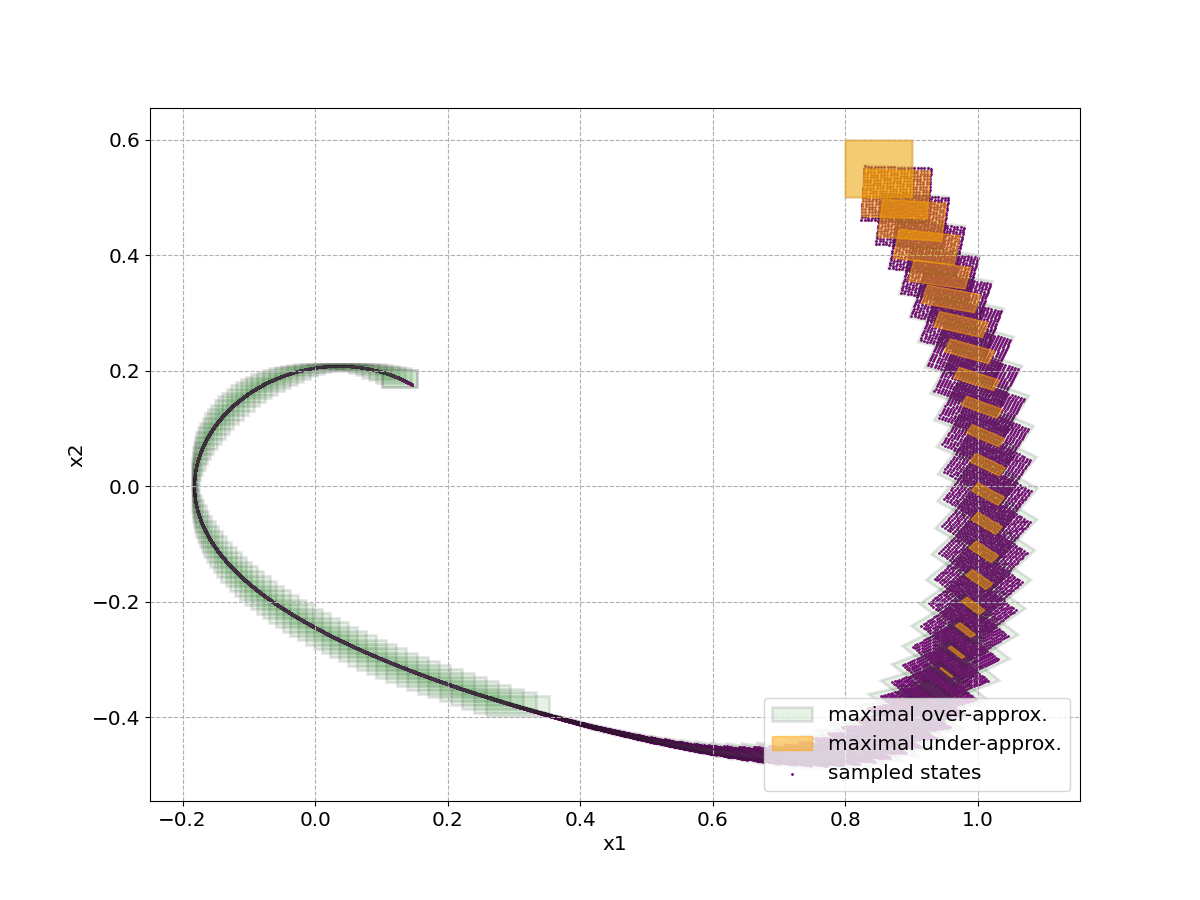
\includegraphics[width=.99\linewidth]{x1x2_approx_sample_B1sig.png}
\caption{ x1x2\_approx\_sample.png for the B1 example}
\label{fig:Proj_sample_B1}
\end{figure}

\section{License}

This project is licensed under the GNU LGPLv3 license - see the \url{https://github.com/cosynus-lix/RINO/blob/master/LICENSE} file for details.

%\begin{figure}
%\centering
%\includegraphics[width=0.3\textwidth]{frog.jpg}
%\caption{\label{fig:frog}This frog was uploaded via the file-tree menu.}
%\end{figure}


%\begin{table}
%\centering
%\begin{tabular}{l|r}
%Item & Quantity \\\hline
%Widgets & 42 \\
%Gadgets & 13
%\end{tabular}
%\caption{\label{tab:widgets}An example table.}
%\end{table}



\bibliographystyle{alpha}
\bibliography{rino}

\end{document}
